\documentclass[11pt]{article}

% basic packages
\usepackage[margin=1in]{geometry}
\usepackage[pdftex]{graphicx}
\usepackage{amsmath,amssymb,amsthm}
\usepackage{custom}
\usepackage{lipsum}

\usepackage{xcolor}
\usepackage{tikz}

\usepackage[most]{tcolorbox}

% page formatting
\usepackage{fancyhdr}
\pagestyle{fancy}

\renewcommand{\sectionmark}[1]{\markright{\textsf{\arabic{section}. #1}}}
\renewcommand{\subsectionmark}[1]{}
\lhead{\textbf{\thepage} \ \ \nouppercase{\rightmark}}
\chead{}
\rhead{}
\lfoot{}
\cfoot{}
\rfoot{}
\setlength{\headheight}{14pt}

\linespread{1.03} % give a little extra room
\setlength{\parindent}{0.2in} % reduce paragraph indent a bit
\setcounter{secnumdepth}{2} % no numbered subsubsections
\setcounter{tocdepth}{2} % no subsubsections in ToC


%%%%%%%%%%%%%%%%%%%%%%%%%%%%%%%%%%%%%%%%%%%%%%%%%%%%%%%%%%%%%%%%%
% CUSTOM BOXES AND STUFF
\newtcolorbox{redbox}{colback=red!5!white,colframe=red!75!black}
\newtcolorbox{bluebox}{colback=blue!5!white,colframe=blue!75!black}
%%%%%%%%%%%%%%%%%%%%%%%%%%%%%%%%%%%%%%%%%%%%%%%%%%%%%%%%%%%%%%%%%


\begin{document}

% make title page
\thispagestyle{empty}
\bigskip \
\vspace{0.1cm}

\begin{center}
{\fontsize{22}{22} \selectfont Physics Directed Reading Program}
\vskip 16pt
{\fontsize{36}{36} \selectfont \bf \sffamily Topology and Geometry in Physics}
\vskip 24pt
{\fontsize{18}{18} \selectfont \rmfamily Keshav Balwant Deoskar} 
\vskip 6pt
{\fontsize{14}{14} \selectfont \ttfamily kdeoskar@berkeley.edu} 
\vskip 24pt
\end{center}

% {\parindent0pt \baselineskip=15.5pt \lipsum[1-4]} 

% make table of contents
% \newpage

These are some notes from the Phyiscs Directed Reading Program (PDRP) group headed by graduate student Vi Hong. Our group was interested in learning about topology and geometry with applications (primarily) to condensed matter physics.   

\vskip 0.5cm
I'm writing these notes primarily to flesh out my own understanding, and so there's some content I've added which may not have actually been covered in the reading group. The order of topics may also be slightly different.

\vskip 0.5cm
\begin{redbox}
    Please feel free to point out and errors / suggestions if you spot any via email! There's likely to be at least a few. 
\end{redbox}

% \microtoc
\tableofcontents 

% main 

%%%%%%%%%%%%%%%%%%%%%%%%%%%%%%%%%%%%%%%%%%%%%%
\newpage
\section{Review of Topology}
%%%%%%%%%%%%%%%%%%%%%%%%%%%%%%%%%%%%%%%%%%%%%%
\vskip 0.5cm


%%%%%%%%%%%%%%%%%%%%%%%%%%%%%%%%%%%%%%%%%%%%%%
\newpage
\section{Path Integrals and Functional Quantization}
%%%%%%%%%%%%%%%%%%%%%%%%%%%%%%%%%%%%%%%%%%%%%%
\vskip 0.5cm

\subsection{The two main approaches to QFT}
Quantum Field Theory (QFT) is often said to be the merger of quantum mechanics and special relativity, but it can be thought of more generally as the "Calculus of infinitely many degrees of freedom" \cite{232AdiscussionNotes}. 

\vskip 0.5cm
In it we deal with fields over spacetime i.e. smooth functions $\phi \text{ : } M \rightarrow N$ where $M$ is our space-time manifold and $N$ some target space, but which are quantized.

\vskip 0.5cm
There are two main approaches one can take to QFT:

\begin{itemize}
    \item \textbf{"Canonical" or "Second" Quantization:} In Quantum Mechanics, our dynamical variables and observables are promoted operators whose measured valued are quantized. 
    
    % In Second Quantization, our dynamical variables are instead treated as \emph{labels} and for each measurable quantity we have a corresponding \emph{field} which gets quantized.

    In Canonical Quantization, we instead think of Fields as being the fundamental constituents of the universe, and of particles as just being bundles of energy or momenta of the corresponding field \cite{Weinberg97}.
    
    In this formulation, a central object of study is the \emph{exponential of the Interaction Hamiltonian}. The exponential of an operator is defined in terms of an expansion, and so this formulation of QFT lends itself to perturbative situations. 
    
    \item For non-perturbative settings like QCD, the \textbf{Path Integral Formulation} serves us better. It also more easily lets us view the relations between QFT, Statistical Physics, and critical phenomena \cite{Maggiore05}.
\end{itemize}

\vskip 0.5cm
\subsection{Heauristic view of Path Integrals}

\vskip 0.5cm
\begin{center}
    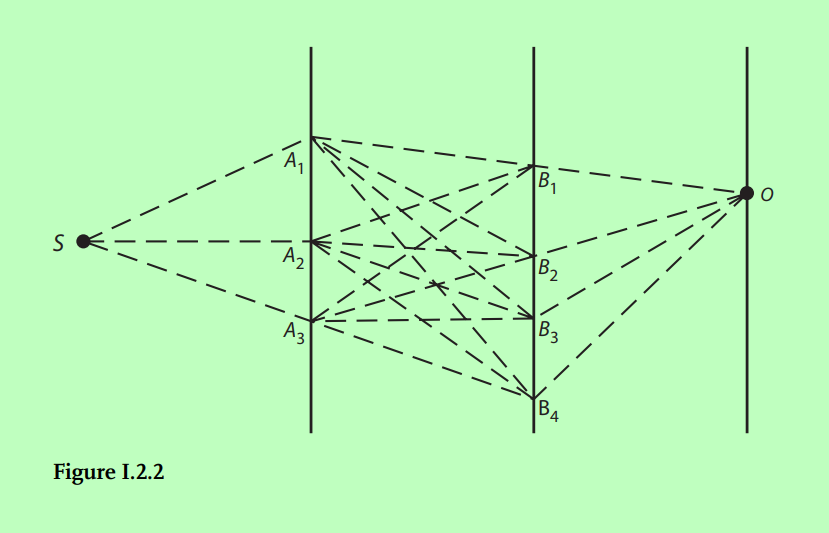
\includegraphics[scale=0.5]{multiple_slits.png}
\end{center}


\vskip 0.5cm
\subsection{Functional Derivatives}

\vskip 0.5cm
\subsection{A... Slightly Less Heauristic View of Path Integrals}



%%%%%%%%%%%%%%%%%%%%%%%%%%%%%%%%%%%%%%%%%%%%%%
\newpage
\section{Fiber Bundles and Principal G-Bundles}
%%%%%%%%%%%%%%%%%%%%%%%%%%%%%%%%%%%%%%%%%%%%%%
\vskip 0.5cm


%%%%%%%%%%%%%%%%%%%%%%%%%%%%%%%%%%%%%%%%%%%%%%
\newpage
\section{Connections on Bundles}
%%%%%%%%%%%%%%%%%%%%%%%%%%%%%%%%%%%%%%%%%%%%%%
\vskip 0.5cm


%%%%%%%%%%%%%%%%%%%%%%%%%%%%%%%%%%%%%%%%%%%%%%
\newpage
\section{Connection 1-forms}
%%%%%%%%%%%%%%%%%%%%%%%%%%%%%%%%%%%%%%%%%%%%%%
\vskip 0.5cm


%%%%%%%%%%%%%%%%%%%%%%%%%%%%%%%%%%%%%%%%%%%%%%
\newpage
\section{TQFTs I}
%%%%%%%%%%%%%%%%%%%%%%%%%%%%%%%%%%%%%%%%%%%%%%
\vskip 0.5cm


%%%%%%%%%%%%%%%%%%%%%%%%%%%%%%%%%%%%%%%%%%%%%%
\newpage
\section{TQFTs II}
%%%%%%%%%%%%%%%%%%%%%%%%%%%%%%%%%%%%%%%%%%%%%%
\vskip 0.5cm


%%%%%%%%%%%%%%%%%%%%%%%%%%%%%%%%%%%%%%%%%%%%%%
\newpage
\section{BRST Quantization}
%%%%%%%%%%%%%%%%%%%%%%%%%%%%%%%%%%%%%%%%%%%%%%
\vskip 0.5cm


%%%%%%%%%%%%%%%%%%%%%%%%%%%%%%%%%%%%%%%%%%%%%%
\newpage
% \section{References}
%%%%%%%%%%%%%%%%%%%%%%%%%%%%%%%%%%%%%%%%%%%%%%
\vskip 0.5cm
\bibliographystyle{plain} % We choose the "plain" reference style
\bibliography{refs} % Entries are in the refs.bib file


\end{document}